Particles produced in the pp collisions traverse through the detector and interact with the detector sub-components in a characteristic manner. Thus, it is possible to reconstruct the corresponding event and identify the types of particles which actually emerged from the collision. \\
The approach for the event reconstruction and identification of specific particles used in CMS is discussed in this Chapter. First, the \textit{Particle-Flow (PF) algorithm} used for a global description of the collision event is introduced. Beyond that, in particular the reconstruction of jets is discussed in Section~\ref{sec:jets_reco}. Furthermore, the identification of decays from b-hadrons and boosted top quarks is reviewed in Sections~\ref{sec:btagging} and~\ref{sec:boosted_tops}, respectively.
\section{Global Event Description with the Particle-Flow Algorithm at CMS}
\label{sec:pf_algo}
The CMS experiment introduced the Particle-Flow algorithm for the reconstruction of collision events. This algorithm is designed to identify all stable particles in an event and can be applied to data events as well as to simulated events in an identical manner. Electrons and photons, charged and neutral hadrons as well as muons are thereby distinguishable and all sub-components of the detector are used by the PF algorithm to reconstruct the particles four-momenta. The CMS detector is very well suited for this task. The silicon tracker enclosed by the uniform magnetic field enables a very efficient track reconstruction yielding only a small track fake rate down to small transverse momenta of $150$\,MeV/c. Furthermore, the strength of the magnetic field together with a high ECAL granularity allows photons to be separated from charged-particle energy deposits. A detailed introduction to the PF algorithm can be found in~\cite{CMS-PAS-PFT-09-001}. \\ 
The event reconstruction starts with the identification of fundamental objects in the sub-detectors which are charged-particle tracks, calorimeter clusters and muon tracks. Tracks emerging from charged particles are formed following an iterative tracking algorithm~\cite{Adam:934067}. Starting from an initial seed trajectory, tracks are extrapolated to further tracker layers by taking into account multiple scattering and energy loss in the material following the equations of motion of a charged particle in a constant magnetic field. Each step proceeds with a removal of unambiguously allocated hits from the previous iteration. With this approach a high tracking efficiency as well as a low fake track rate can be achieved which is a crucial requirement for a successful particle-flow event reconstruction. Furthermore, calorimeter clusters are formed in each sub-detector separately based on adjacent calorimeter cells. Neighbouring cells are combined to form clusters when their energy exceeds a pre-defined threshold. \\
A particle traversing through the detector gives typically rise to several of such elementary components so that a dedicated link algorithm is applied in order to connect these elements and form blocks while removing a potential double-counting of the same object in different detector parts. First, charged-tracks are associated to calorimeter clusters, if the extrapolated trajectory matches the cluster within the cluster boundaries. This is done considering effects like gaps and cracks between detector components, uncertainty on the shower position or multiple-scattering. Photons from Bremsstrahlung are considered by extrapolating also tangents of the tracks to the respective energy clusters. In a similar manner ECAL and HCAL clusters can be connected to each other as well by linking clusters in the more granular calorimeter to clusters in the less granular one. At last global muons can be defined by associating charged-tracks from the tracker with muon tracks reconstructed in the muon system. \\
After the identification of such blocks of elements the PF algorithm proceeds to finally create a list of all particles contained in the event applying dedicated quality criteria interpreting the blocks in terms of particles. The identification of muons and a removal of their tracks from the blocks is followed by an assignment of electrons and associated Bremsstrahlung from tracks and linked ECAL clusters. After these have been removed from the list of blocks as well, remaining good quality tracks are considered to be charged hadrons. Their momenta are determined from combining the track momentum and the respective energy in the calorimeter cluster. If the cluster energy largely exceeds the measured momentum from the track beyond the detector resolution, it constitutes a photon and if the excess is larger than the total ECAL energy also a neutral hadron. Finally, remaining ECAL and HCAL clusters not linked to any track give rise to photons and neutral hadrons. \\
The complete set of particles can then be used to derive further objects and quantities like e.g. jets as discussed in Section~\ref{sec:jets_reco}, missing transverse energy $E_{T}^{\mathrm{miss}}$ which is the magnitude of the vector momentum imbalance perpendicular to the beam direction or decay products of tau leptons. More detailled information on the specific quality criteria required for the identification of certain particles is given in the Chapters~\ref{chap:Resolution},~\ref{chap:RA2} and~\ref{chap:Stop} for each analysis presented in this thesis, individually.

\section{Reconstruction of Jets}
\label{sec:jets_reco}
As stated already earlier jets are the experimental signatures of quarks and gluons and constitute of a collimated spray of hadrons. However, in order to identify a particular jet and relate its properties to the original parton a proper jet definition is needed. Typically, a \textit{jet algorithm} determines how to cluster particles into a jet. Furthermore, it has to be defined how to assign a momentum to the jet. At CMS, the standard procedure is to assign the four-momentum sum of all jet constituents to the jet. \\
Different jet algorithms are introduced in Section~\ref{subsec:jets_algos} followed by a discussion of different jet types used at CMS in Section~\ref{subsec:jets_types}. Furthermore, the jet transverse-momentum response is defined in Section~\ref{subsec:jets_response} and the calibration of jet energies is reviewed in Section~\ref{subsec:jets_calib}.
\subsection{Jet Algorithms}
\label{subsec:jets_algos}
\begin{figure}[!tp]
  \centering 
  \begin{tabular}{cc}
    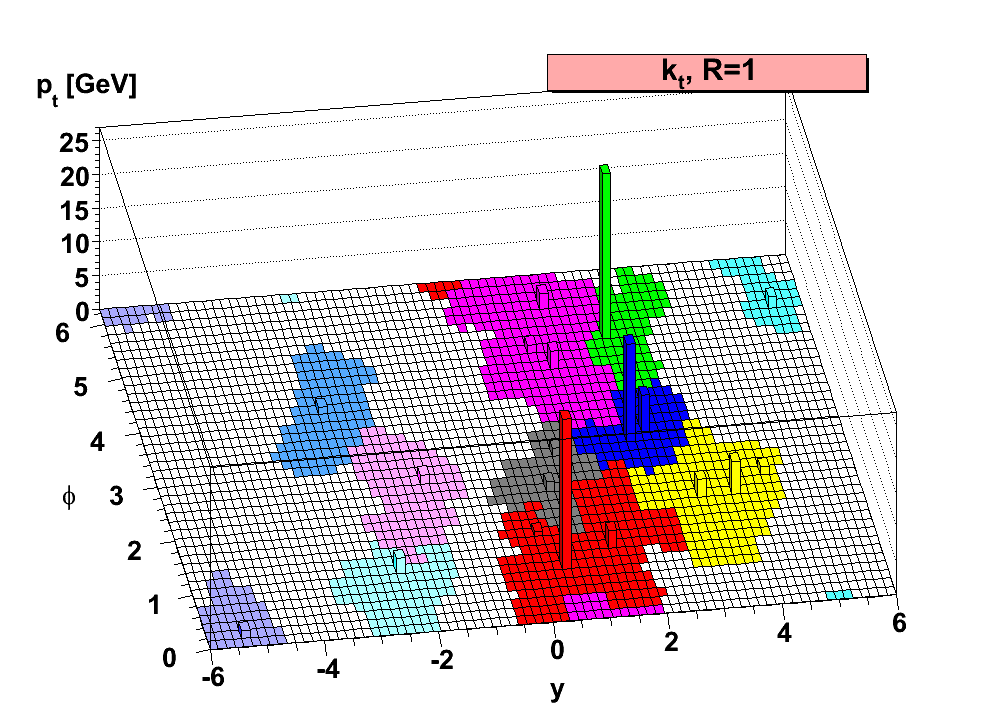
\includegraphics[width=0.49\textwidth]{figures/herwig-parton-level-ev-kt.png} &
    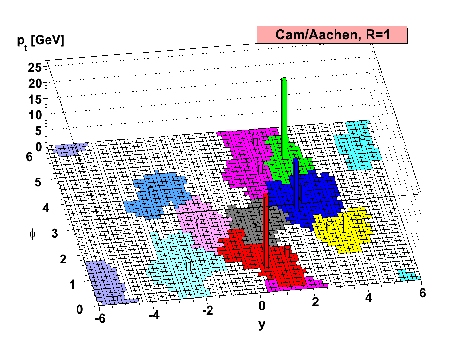
\includegraphics[width=0.49\textwidth]{figures/herwig-parton-level-ev-cam.png} \\
    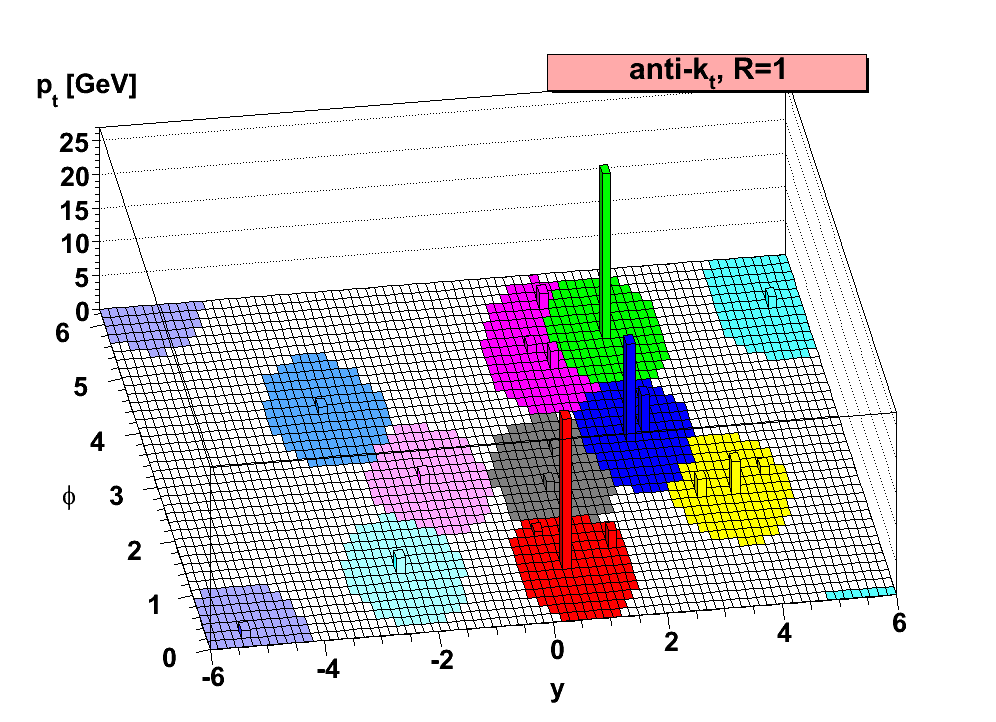
\includegraphics[width=0.49\textwidth]{figures/herwig-parton-level-ev-antikt.png} &
    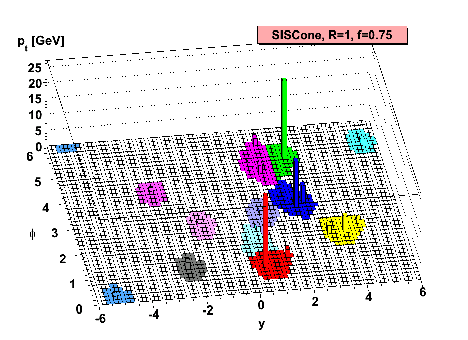
\includegraphics[width=0.49\textwidth]{figures/herwig-parton-level-ev-siscone.png}   
  \end{tabular}
  \caption{Sample parton-level event generated with \herwig, adding many random soft particles, that is clustered with the $\mathrm{k_T}$ -algorithm (\textit{top left}), the C/A-algorithm (\textit{top right}), the SISCone-algorithm (\textit{bottom left}) and the $anti-\mathrm{k_{T}}$-algorithm (\textit{bottom right}). Colours illustrate the active areas of the resulting hard jets. Taken from~\cite{Salam:2009jx}.}
  \label{fig:jet_algos}
\end{figure}
A jet algorithm usually provides a prescription how to combine individual particles into a single jet based on some distance criterium. Good jet algorithms though should be able to identify jets that are neither sensitive to the emission of soft particles (\textit{infrared safety}) nor to the collinear splitting of particles (\textit{collinear safety}). These features named \textit{IRC safety} are desirable as otherwise e.g. cross sections would be dependent on particular effects of hadronisation involving random collinear splittings and soft emissions making it difficult to compare the results from experiments to theroretical predictions. This effect is even enforced because detectors intrinsically provide regularisation of IRC effects to some extent due to a finite resolution. Furthermore, calculations in QCD perturbation theory rely on the cancellation of divergences related to IRC processes. Thus, if jets are sensitive to such effects cancellations are not ensured and can lead to inifinite cross sections. \\
An introduction to the most commonly used jet algorithms known as \textit{cone algorithms} and \textit{sequential recombination algorithms} is given in the following. A comprehensive overview of jet algorithms and properties can be found in~\cite{Salam:2009jx}.
\begin{description}
 \item \textbf{Cone Algorithms:} Cone algorithms were the first developed jet algorithms. They are based on the general idea that the main kinematics in an event are not changed by specific effects from hadronisation and thus a jet is defined by a set of particles within a stable cone around their centre of mass. Typically, separate angular or energy parameters are used to perform the jet finding. A very common approach is implemented in \textit{iterative cone} (IC) algorithms. Here, a seed constituent $i$ which is for instance the constituent with the highest transverse momentum defines the initial direction and momenta of all constituents $j$ within a cone defined by
\begin{equation}
 \Delta R_{i,j}^2 = (\eta_i - \eta_j)^2 + (\phi_i - \phi_j)^2 < R^2
\end{equation}
are added to the momentum of the seed. The resulting direction is used as new seed direction and the whole procedure is repeated until a stable cone is achieved. The dimensionless parameter $R$ hence defines the jet radius. After the finding of such a jet, all constituents are removed from the input list and further jets are clustered from the remaining objects. This progressive removal approach avoids to form jets with overlapping cones. However, such a procedure is not IRC safe as collinear splittings can lead to different final ensembles of jets. \\
The issue with IRC safety in cone algorithms can be avoided by instead of iteratively forming stable cones one after the other identifying all stable cone solutions at once. This procedure is denoted \textit{seedless cone} (SC) algorithm. The usage of such algorithms though is typically impractical as the computation time increases exponentially with the number of particles to be considered so that even for 100 particles it is not solveable at any reasonable timescale. A feasible implementation of a seedless cone algorithm featuring only a logarithmic time-dependence is given by the SISCone algorithm~\cite{Salam:2007xv}. As it is usually nonetheless still more time consuming than sequential algorithms as described in the next part, the SISCone algorithm is not used by CMS.
 \item \textbf{Sequential Recombination Algorithms:} The basic concept of sequential clustering algorithms is to group in an iterative procedure pairs of particles together based on some distance measure and thus reconstructs to some extent the evolution of a parton shower. A suitable metric to be used at hadron colliders where the total energy of a collision is unknown based on variables invariant under longitudinal boosts is 
\begin{equation*}
d_{ij} = \mathrm{min}(k_{T,i}^{2p}, k_{T,j}^{2p}) \frac{\Delta R_{ij}^2}{R^2}
\end{equation*}
\begin{equation*}
d_{iB} = k_{T,i}^{2p}
\end{equation*}
with the distance $d_{ij}$ between final state objects $i$ and $j$ carrying transverse momentum $k_T$ and the distance of the object to the beam $d_{iB}$. While $\Delta R_{ij}$ denotes the spatial separation in the $(\eta, \phi)$-plane, $R$ and $p$ are free parameters of the algorithm. The recombination is done by first calculating $d_{ij}$ and $d_{iB}$ for all objects in the final state by identifying the minimum value. If the minimum is $d_{ij}$, the two objects $i$ and $j$ are combined and all distances are computed again. However, if the minimum is $d_{iB}$, object $i$ is declared a jet and removed from the input list. This procedure is repeated until all objects are assigned. In this context the parameter $R$ acts as an angular cut-off and thus has a similar role as the jet radius in cone algorithms. Depending on the choice of the parameter $p$ different types of algorithms are distinguished which are all IRC safe. An illustration of an arbitrary example event where jets are clustered with the different jet algorithms is shown in Fig~\ref{fig:jet_algos}. The $k_T$-algorithm uses $p = 1$~\cite{PhysRevD.48.3160} and thus clusters soft particles first. This results mainly in irregular shaped jets (cf. Fig~\ref{fig:jet_algos}) and makes them sensitive to radiation in the event. Consequently, they are difficult to calibrate and therefore impratical to use at hadron colliders. The \textit{Cambride-Aachen}- or short \textit{CA}-algorithm~\cite{Dokshitzer:1997in, Wobisch:1998wt} utilizes $p = 0$. Thus, it does not rely on momentum information but clusters jets based on the angular separation of input objects. This allows a direct geometric interpretation of jets and makes this type of jet algorithm especially suited for analyses of jet substructure as will be discussed later in Section~\ref{sec:boosted_tops}. These jets do still reflect the structure of the parton shower, but are less affected by soft radiation than the $k_T$-algorithm. Finally, the \textit{anti-$k_T$}-algorithm uses $p = -1$~\cite{1126-6708-2008-04-063} and starts the jet clustering beginning with the hardest objects in the event. Hence, the evolution of the parton shower is not reproduced. The anti-$\mathrm{k_T}$ algorithm tends to form very regular shaped jets, as the four-momentum of the core of the jet is not much affected by the softer components which are clustered later in the process. Typically, the regular shape allows an easy calibration of anti-$\mathrm{k_T}$ jets. 
\end{description}

\subsection{Jet Types at CMS}
\begin{figure}[!tp]
  \centering 
  \begin{tabular}{c}
    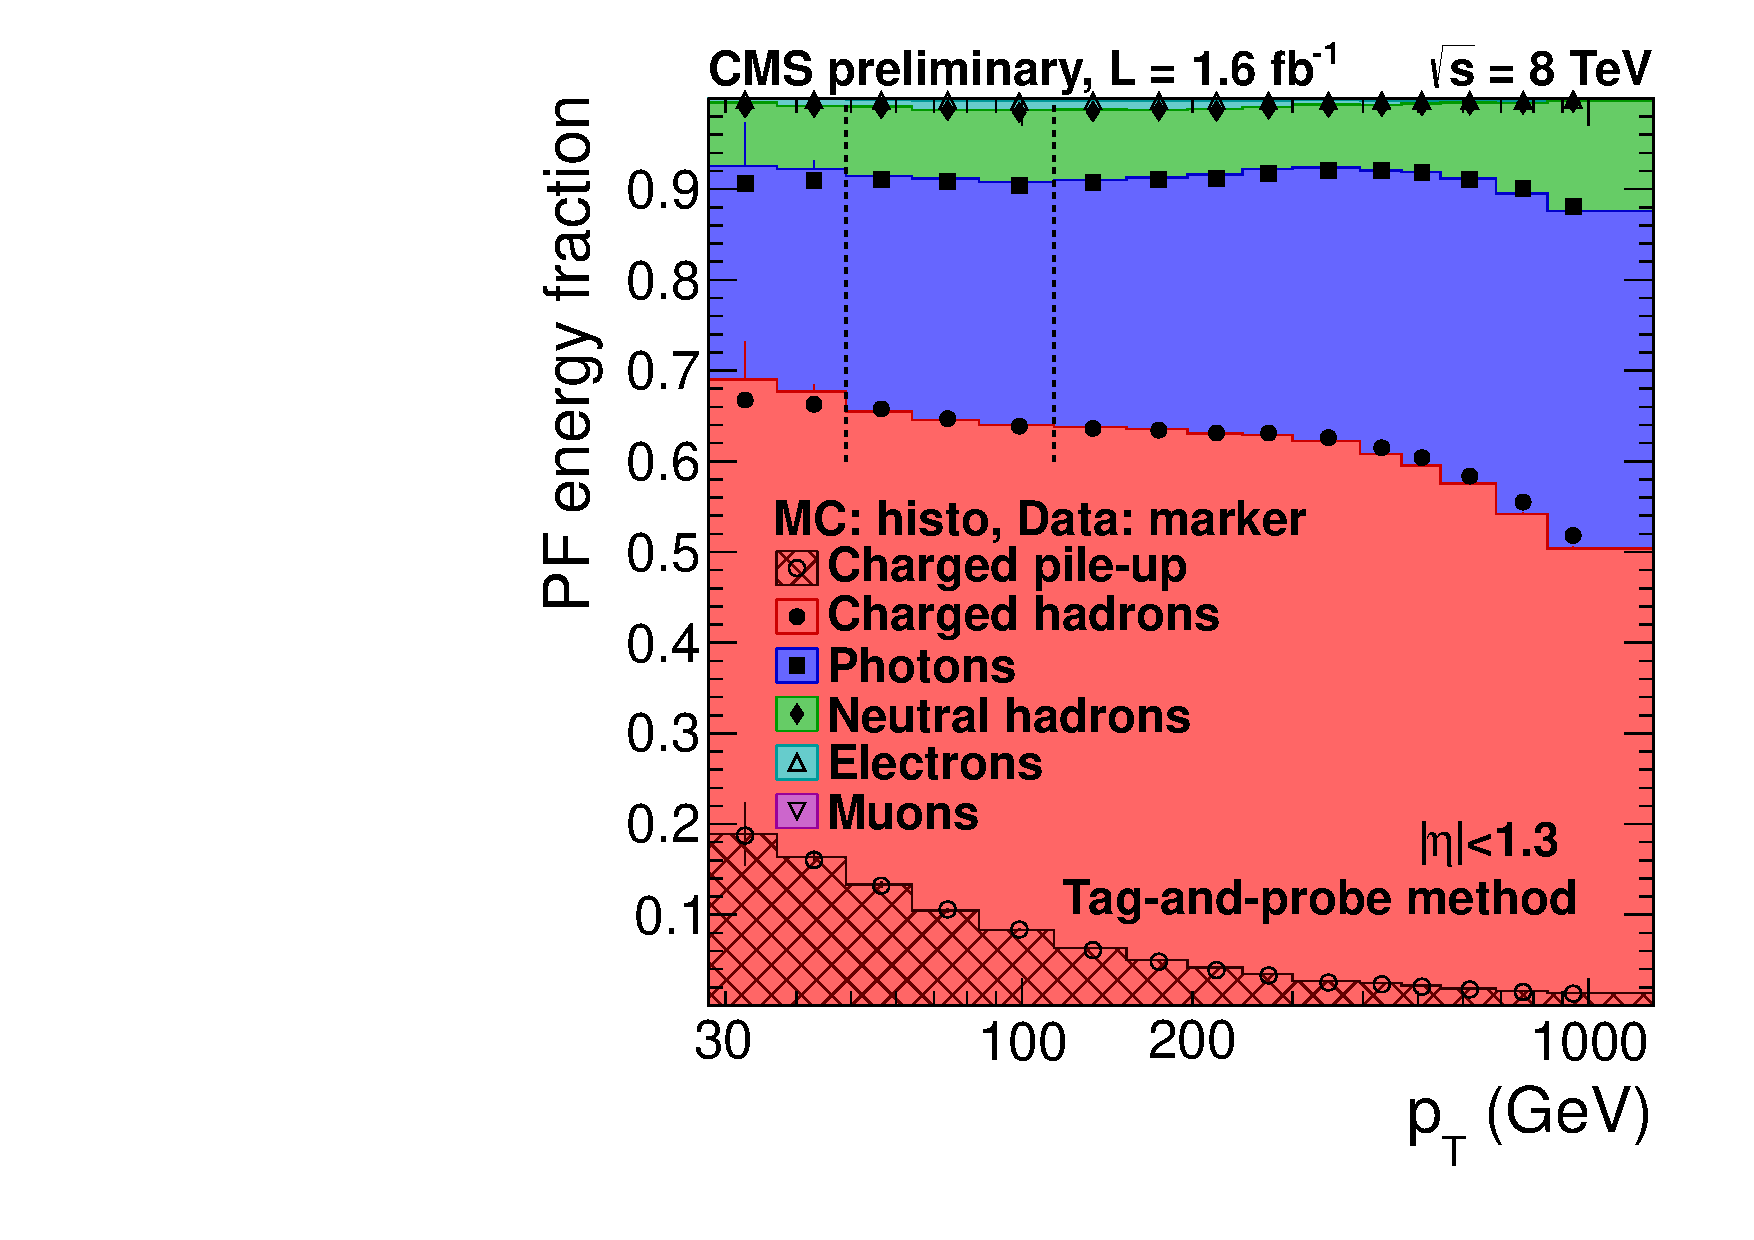
\includegraphics[width=0.6\textwidth]{figures/calcFrac_Frac0_MC-1.pdf} 
  \end{tabular}
  \caption{Composition of the PF jet energy versus jet \pt in the barrel detector region $|\eta| < 1.3$ in simulated events (coloured histograms) and data (solid markers). Taken from~\cite{CMS-DP-2012-012}.}
  \label{fig:jets_pf_comp}
\end{figure}
\label{subsec:jets_types}
The default jets to be used at the CMS experiment are jets clustered by the anti-$\mathrm{k_T}$ algorithm using a distance parameter of R = 0.5. This can be applied to reconstructed detector signals resulting in \textit{detector-level} jets or to final-state particles after hadronisation, as this is possible in simulated events, giving rise to \textit{particle-level} jets. Implementations of various jet algorithms are provided by the \textit{FastJet} package~\cite{Cacciari:2011ma, Cacciari:2005hq}. \\
Based on the information used from the various CMS subdetectors for the jet clustering different types of detector-level jets are distinguished. Some of them are the following~\cite{1748-0221-6-11-P11002}:
\begin{description}
 \item \textbf{Calorimeter (Calo) jets:} Calo jets are clustered from energy deposits in the calorimeters. For this purpose, calormeter towers are defined which consist of at least one HCAL cell and the geometrically associated ECAL cells. In case of the barrel detector region a calorimeter tower consists for instance of one HCAL cell and $\mathrm{5 \times 5}$ ECAL cells. The four-momentum of each tower is defined by the tower position as seen from the interaction point and the energy deposit in the tower above a certain threshold assuming a mass of zero. 
 \item \textbf{Jet-Plus-Track (JPT) jets:} JPT jets are reconstructed from calorimeter jets complemented by tracking information~\cite{CMS-PAS-JME-09-002}. Tracks of charged particles can be associated to calo jets based on the separation of the jet axis and the momentum vector of the track in the $(\eta,\phi)$-plane. Associated tracks are projected to the jet cone and are exploited to correct the jet energy and direction resulting in an improved jet response.
 \item \textbf{Particle-Flow (PF) jets:} PF jets are clustered from the four-momentum vectors of particle-flow candidates as identified by the PF algorithm described in Section~\ref{sec:pf_algo}. Typically, these types of jets show the best performance as the excellent resolution of the tracking system and the ECAL are utilized. Only neutral hadrons which consitute around 15\% of the jet energy (cf. Fig.~\ref{fig:jets_pf_comp}) rely on the energy measurement of the HCAL with its relatively poor resolution. Thus, PF jets are the default jets to be used at the CMS experiment, as it is done within this thesis. In order to mitigate influences from pile-up, charged hadrons unambigously associated to vertices other than the primary vertex can be subtracted from the event before performing the actual jet clustering. This technique is referred to as \textit{charged hadron subtraction} (CHS) and used as default throughout this thesis. 
\end{description}

\subsection{Jet Transverse-Momentum Response}
\label{subsec:jets_response}
In general, the jet transverse momentum as measured at detector level is not necessarily equal to the energy of the original particle due to for instance the limited detector resolution. This effect is quantified by the \textit{jet transverse-momentum response} R which is defined as 
\begin{equation}
  \mathrm{R} = \frac{\pt}{\pt^{\mathrm{particle}}} 
  \label{eq:response}
 \end{equation}
where \pt denotes the transverse momentum of the jet measured at detector level and $\pt^{\rm{particle}}$ is the transverse momentum of the original particle-level jet. Thus, the jet response provides a measure of the fraction of the jet momentum visible in the detector compared to the actual momentum of the particle after hadronisation. \\
The average response $\langle R \rangle$ is referred to as \textit{jet energy scale} (JES) and has to be calibrated such that $\langle R \rangle = 1$ for fixed $\pt^{\mathrm{particle}}$. The response usually depends on the jet momentum as well as on the pseudorapidity. This is expected since the quality of the jet measurement is directly related to the energy of the particles and the resolution of the detector sub-components. This is for instance caused by the specific track-reconstruction efficiency or the individual amount of detector material. \\
Furthermore, the width of the response distribution corresponds to the relative \textit{jet transverse-momentum resolution} (JER) and hence is a function of \pt and $\eta$ as well. 

\subsection{Jet Energy Calibration}
\label{subsec:jets_calib}
In order to relate the measured jet momentum on average to the momentum of the corresponding particle-level jet a jet calibration procedure is applied. Within the CMS experiment a factorized approach is utilized which is described in detail in~\cite{1748-0221-6-11-P11002}. \\
The calibrated jet four-momentum vector $p^{cor}$ is obtained from the raw jet momentum four-vector $p^{raw}$ by scaling the raw momentum with a correction factor $C$ according to
\begin{equation}
p^{cor} = C \cdot p^{raw} = C_{\mathrm{offset}}(\pt^{raw}, \eta) \cdot C_{\mathrm{rel}}(\eta) \cdot C_{\mathrm{abs}}(\pt') \cdot C_{res}(\pt'', \eta) \cdot p^{raw}
\end{equation} 
 where $C$ is composed of the offset correction $C_{\mathrm{offset}}$, the calibration factors $C_{\mathrm{rel}}$ and $C_{\mathrm{abs}}$ as well as residual correction factors $C_{\mathrm{res}}$ applied to data. Each correction factor is applied sequentially after the other in a fixed order such that $\pt'$ denotes the transverse momentum after the application of the offset correction and $\pt''$ is the transverse momentum after all previous corrections. Some details for each individual correction are given in the following: 
\begin{description}
 \item \textbf{L1 Offset:} The L1 offset correction is designed to compensate for additional energy contributions arising from instrumental noise or pile-up events. The \pt offset is estimated in dependence of $\eta$, the effective jet area $A_j$ and the \pt-density $\rho$. The jet area is determined by adding a large number of inifinitely small four-momentum vectors to the event. The active jet area is hence defined as the region in the $(\eta, \phi)$-plane occupied by the soft particles after clustering them together with the true hard jet components. The \pt-density $\rho$ is defined on an event-by-event basis as the median of the distribution $\pt^{j}/A_{j}$ where $j$ denotes all reconstructed jets in the event. The offset in \pt is estimated from simulated QCD multijet events by directly comparing the jet momentum of a jet with and without pile-up overlaid.  
 \item \textbf{L2 Relative $+$ L3 Absolute Correction:} The L2 relative correction is designed to make the jet energy scale uniform with respect to $\eta$ while the L3 absolute correction ensures a uniform response versus \pt. Both corrections are entirely estimated from simulated QCD multijet events. The correction is defined as the inverse of the average response $1/\langle R \rangle$.
 \item \textbf{L2L3 Residual Correction:} In order to compensate for remaining response differences between simulated events and data, residual correction factors are derived. These are applied to data only and correct for remaining differences in the data-to-simulation ratio of the relative jet energy scale. Such corrections can be derived from events featuring a momentum balance in the transverse plane like dijet events (used for the L2 residual determination) or $\mathrm{Z/\gamma+jet}$ events (used for the measurement of the L3 residual correction).
\end{description}
The calibration factors are obtained with respect to the average flavour composition of a QCD mulitjet sample. Thus, further steps of correction factors can be applied for specific analysis purposes correcting e.g. the different response for various jet flavours.  However, such higher order corrections are not used in this thesis. \\ 
The actual set of correction factors used in this thesis, if not stated otherwise, is documented in~\cite{CMS-DP-2013-033} and illustrated in Fig. ... \todo{Fig. JEC}. In total, the size of the JES corrections are at the order of ... \todo{size of JEC}.

\section{Identification of b-Quark Jets}
\label{sec:btagging}
Jets arising from the hadronization of bottom quarks are usually referred to as \textit{b-jets}. As these are existent in many physics processes as e.g. the decay of top quarks, it is of essential importance to be able to identify b jets and distinguish them from jets initiated by gluons or light-flavour quarks. Typically, the identification of b-jets is denoted \textit{b-tagging} and the distinct properties of b quarks are exploited for the identification of the respective jets. In general, hadronic jets arising from the fragmentation of b quarks possess quite large masses, long lifetimes and daughter particles featuring hard momentum spectra. The CMS experiment with the ability to perform a precise charged-particle tracking and lepton identification exploits the specific b jet properties in dedicated b-tagging algorithms for an efficient b-jet identification~\cite{Chatrchyan:2012jua}:
\begin{description}
 \item \textbf{Track Counting (TC) algorithm:} A powerful discriminator for the decay products of a b hadron from prompt tracks is the \textit{impact parameter} (IP) of a track with respect to the primary vertex. Its significance can be computed by taking the ratio of the IP to its respective uncertainty. Tracks in a jet are sorted by decreasing values of the IP significance by the TC algorithm. Depending on whether the IP significance of the second or the third ranked track is chosen as discriminator value the algorithm is denoted \textit{Track Counting High Efficiency} (TCHE) or \textit{Track Counting High Purity} (TCHP) algorithm. 
 \item \textbf{Jet Probability (JP) algorithm:} The JP algorithm extends the simple TC algorithm by connecting the information about the IP from a couple of tracks in the jet. A likelihood is calculated that all tracks of the jet stem actually from the primary vertex. This appraoch can be varied by giving more weight to tracks with the highest IP significance. The maximum of such tracks is four and matches the average number of reconstructed charged particles from the decay of b hadrons. This version is called \textit{Jet B Probability} (JBP) algorithm.
 \item \textbf{Simple Secondary Vertex (SSV) algorithm:} A further useful discriminating feature for b tagging is the presence of a secondary vertex and related kinematic variables like the flight distance and direction which can be determined from the vector between the primary and secondary vertex. The SSV exploits the significance of the flight distance which is given by the flight distance divided by the associated uncertainty. Two different versions of this algorithm exist targeting on the one hand a \textit{High Efficiency} (SSVHE) and on the other hand a \textit{High Purity} (SSVHP). While the SSVHE is based on vertices with at least two associated tracks, the SSVHP uses vertices with more than three tracks. Typically, the efficiency of the algorithm is limited by the reconstruction efficiency of secondary vertices which amounts to about 65\%.  
 \item \textbf{Combined Secondary Vertex (CSV) algorithm:} The CSV algorithm provides an efficient identification of b jets also in cases when no secondary vertex could be recosntructed. It utilizes an approach combining information from secondary vertices as well as track-based lifetime information and thus is able to exceed the efficiency of SSV algorithms. Often, pseudo-vertices can be formed from tracks even when failing the reconstruction of an actual secondary vertex which allows to derive some secondary vertex related quantities. Variables used in the CSV algorithm are e.g. flight distance significance, vertex mass, number of tracks at the vertex, number of tracks in the jet or the IP sigificances for the tracks in the jet. These variables are used to compute two likelihood ratios which can be used to distinguish either c and b jets or light-parton and b jets. 
\end{description}  
Each algorithm determines a discriminator value per jet indicating how b-jet-like a jet behaves. Based on that, working points are defined corresponding to a specific minimum threshold of the discriminator value. These working points are named \textit{loose}, \textit{medium} and \textit{tight} and correspond to a misidentification probability, \ie the probability to identify a non-b jet as b jet, of $10\%$, $1\%$ and $0.1\%$ for an average jet momentum of $80$\gev, respectively. \\
\begin{figure}[!tp]
  \centering 
  \begin{tabular}{cc}
    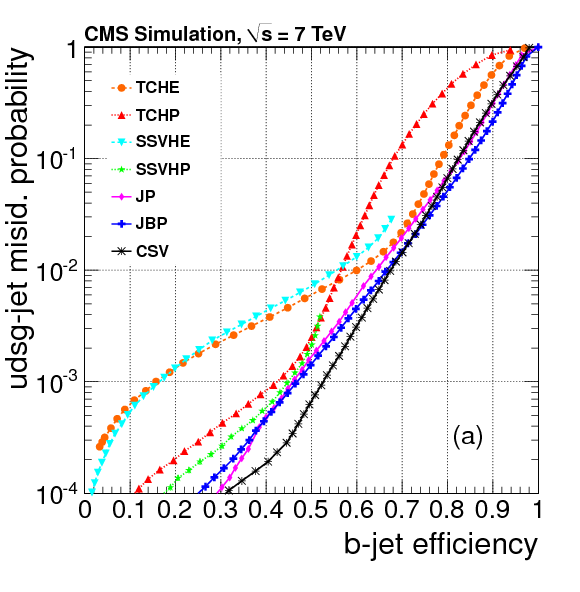
\includegraphics[width=0.49\textwidth]{figures/figAlgo_Combined_udsgvsb_Efficienies.png} &
    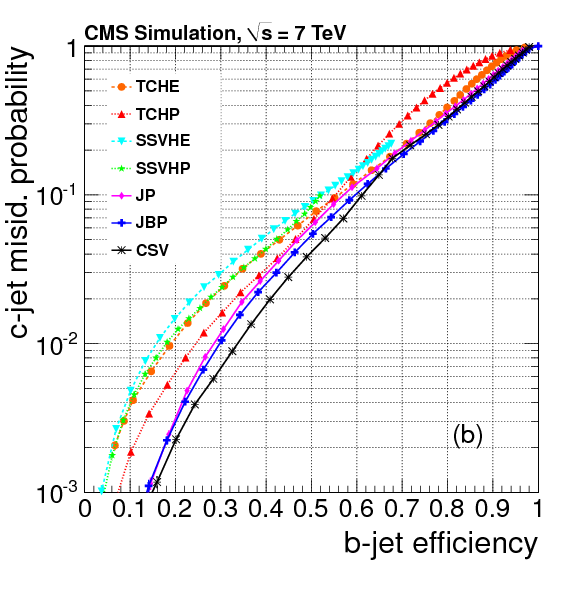
\includegraphics[width=0.49\textwidth]{figures/figAlgo_Combined_cvsb_Efficienies.png} 
  \end{tabular}
  \caption{Performance curves obtained from simulation for the algorithms described in the text. (a) light-parton- and (b) c-jet misidentification probabilities as a function of the b-jet efficiency. Taken from~\cite{Chatrchyan:2012jua}.}
  \label{fig:btagging}
\end{figure}
In order to determine the quality of a particular b-tagging algorithm, typically the misidentification probability as function of the b-tag efficiency is compared for various taggers. Such a performance comparison is illustrated in Fig~\ref{fig:btagging} for the tagging algorithms described above. The misidentification probability is derived separately for light-flavour and gluon initiated jets as well as c-jets. The curves are derived from simulated multijet events using jets with $\pt > 60$\,\gev. For loose working points the b-tag efficiency is around $\approx 80-85\%$ and the JBP algorithm shows the best performance. In case of medium and tight selections, the b-tag efficiency drops to $\approx 45-55\%$ and the CSV algorithm performs best. \\
B-tagging algorithms used for analyses of data obtained at $\sqrt{s} = 8$\tev in 2012 where the TCHP, JP and CSV algorithm~\cite{CMS-PAS-BTV-13-001}. In order to compare the b-tagging performance in data and simulation two different event samples have been selected. On the one hand, an inclusive multijet sample is selected requiring at least one jet with $\pt = 60 - 500$\gev which is dominated by jets from light-flavour quarks and gluons. On the other hand, a sample dominated by top-pair production is selected requiring an electron, a muon and at least two jets with $\pt>30$\gev such that this sample is enriched in b-jets. These samples allow to compare quantities relevant for b-tagging in data and simulation like e.g. the number of secondary vertices or b-tag discriminator values. In general, quantities relevant for b-tagging show a good agreement between data and simulation with deviations within 20\%. Typically, efficiencies and misidentification probabilities are measured as function of jet transverse momentum and pseudorapidity. A potential disagreement between data and simulation can be expressed in terms of \textit{scale factors} and corrected for in analyses such that b-tagging efficiency and misidentification probability in data and simulation match. 

\section{Identification of Boosted t-Quark Jets }
\label{sec:boosted_tops}
Supersymmetric models or other scenarios describing physics beyond the Standard Model predict the extistence of new massive particles. Often, the coupling of these particles especially to quarks belonging to the third generation is sizeable like e.g. in decays of top squarks which predominantly are expected to decay into top quarks. Consequently, such processes lead to highly-energetic top-quarks in the final state which can be identified exploiting the specific properties of the top-quark. \\
\begin{figure}[!tp]
  \centering 
  \begin{tabular}{c}
    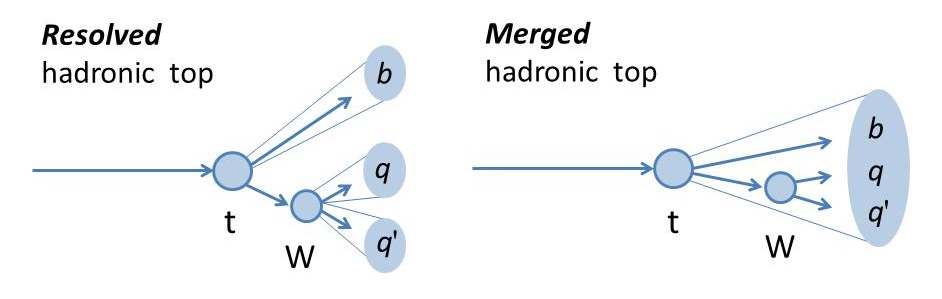
\includegraphics[width=1.0\textwidth]{figures/BoostedTops.jpg} 
  \end{tabular}
  \caption{Schematic diagrams of the decay of a top-quark in the resolved case (\textit{left}) and the boosted scenario (\textit{right}).}
  \label{fig:boosted_top}
\end{figure}
The top-quark is the heaviest quark with a mass of $173.34 \pm 0.76$\gev~\cite{ATLAS:2014wva} resulting in a rapid decay. This decay happens even faster than the hadronisation timescale is such that the top-quark behaves in the detector as a bare quark without forming color-neutral hadrons. The decay takes place via the weak interaction and as denoted in Sec.~\ref{sec:sm}, the quark mixing is parametrized by the CKM-matrix. Since the corresponding matrix element $V_{\mathrm{tb}} \approx 1$, the top quark decays thus almost exclusively into a W boson and a b-quark. Therefore, the decay of the top-quark is strongly characterized by the decay of the W boson. In general, the W boson can decay into a charged lepton and its corresponding neutrino or a pair of light quarks which are up, down, charm and strange. Taking into account the three possible colour states for eack quark pair this results in nine different W decay modes. Consequently, two thirds of top quark decays result exclusively in hadrons which is typically referred to as \textit{hadronic top}. If top quarks are produced with low energy ($< 2 m_{t}$), the decay will predominantly occur at rest and the top decay products show up as three distinct signatures in the detector. In the case of hadronic tops these are three well separated jets. However, if the top transverse momentum is high, the decay products are \textit{boosted} and thus collimated in the forward direction. Consequently, they might overlap and merge into a single large jet (\textit{fat jet}). The opening angle of the decay products $\Delta R$ is expected to scale as
\begin{equation}
 \Delta R \approx 2\,m /p_{T}
\end{equation}  
where m and \pt are the mass and the transverse momentum of the decaying particle, respectively. Schematic diagrams of resolved and boosted top quark decays are illustrated in Fig.~\ref{fig:boosted_top}. The identification of boosted top-quark decays -- here restricted to hadronic tops -- is typically known as \textit{top tagging} and aims at the determination of the decay
\begin{equation}
 t \rightarrow W + b \rightarrow qq' + b 
\end{equation} 
by analysing the substructure of fat jets and applying kinematic selections\todo{jet grooming}. \\ 
Within the CMS experiment several top tagging algorithms (or short \textit{taggers}) are commissioned~\cite{CMS:2014fya, CMS-DP-2014-036}. Two of them are described in some detail in the following:
\begin{description}
\begin{figure}[!tp]
  \centering 
  \begin{tabular}{cc}
    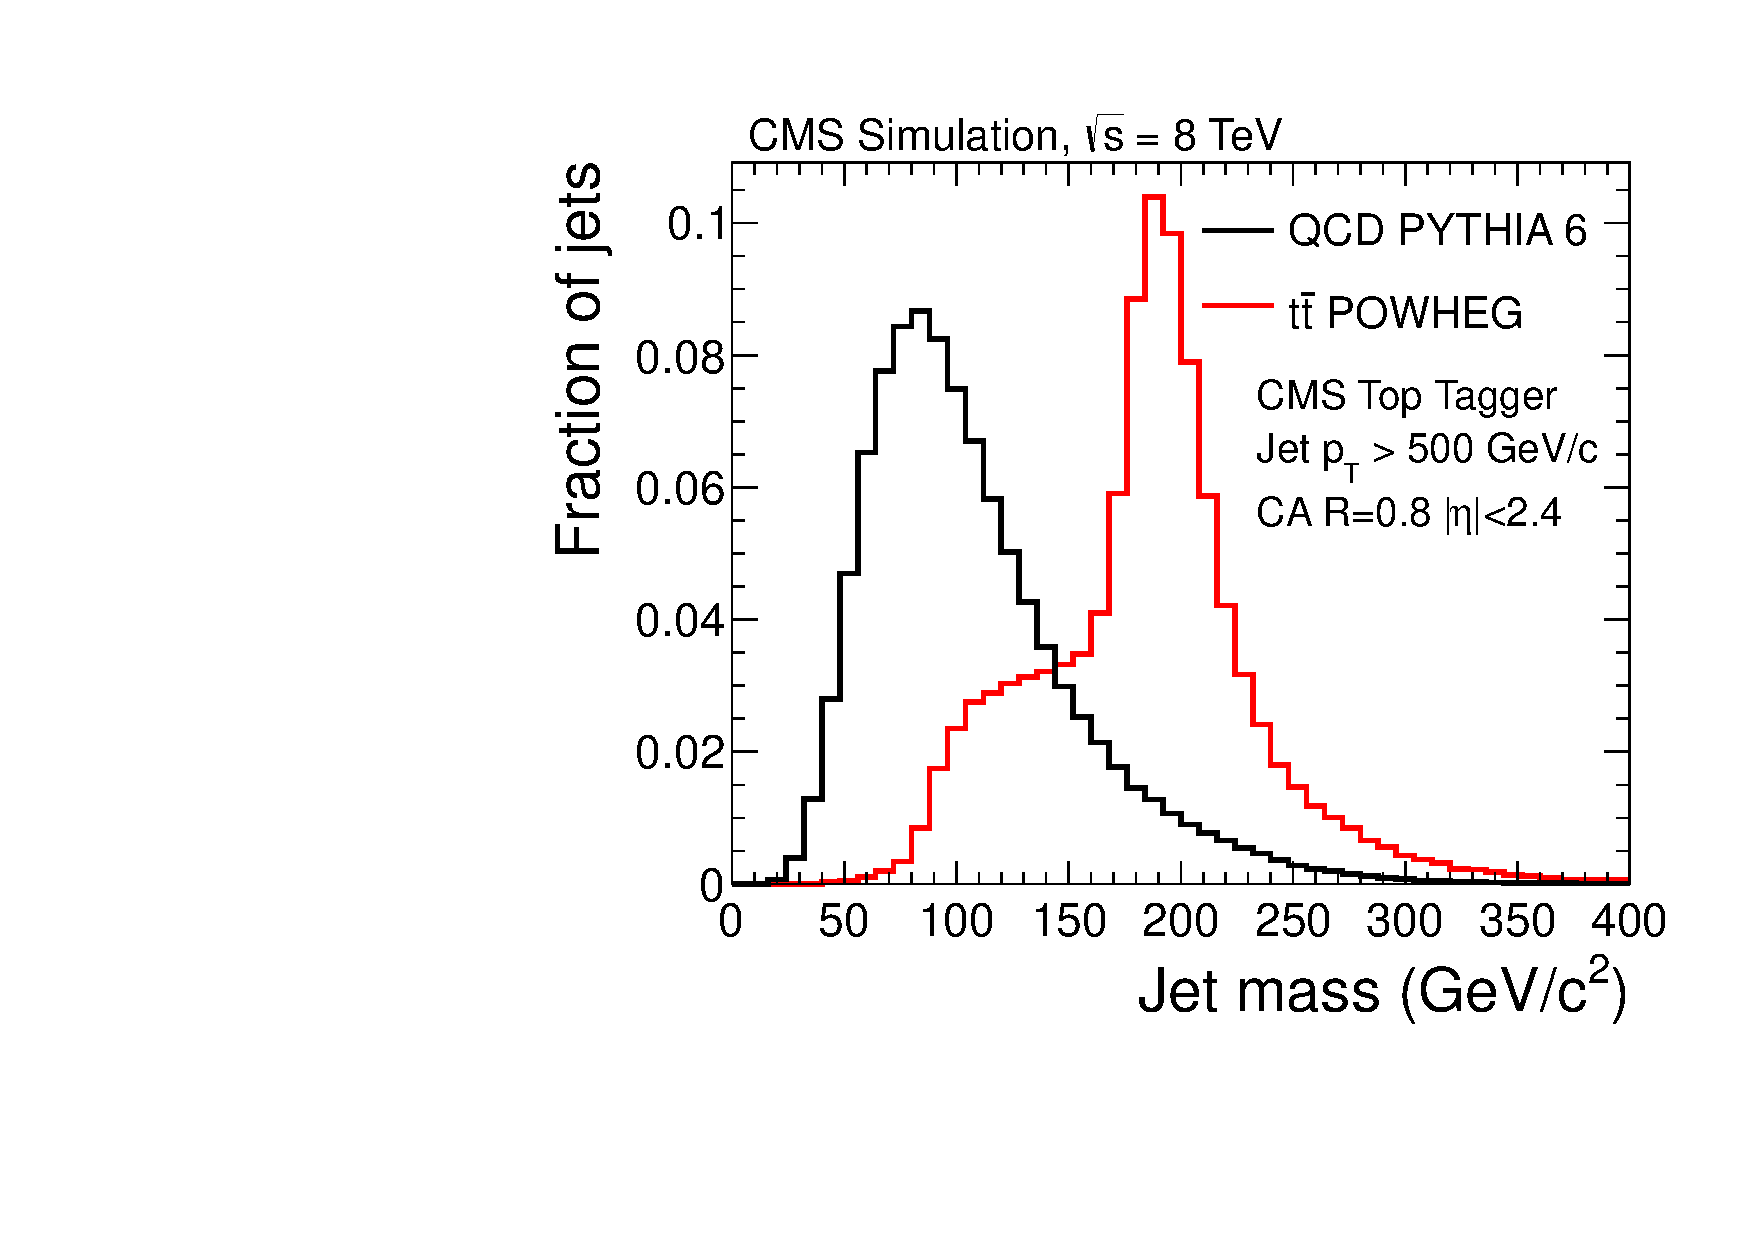
\includegraphics[width=0.49\textwidth]{figures/Draw2HistogramsFrom1File_QQ_MASS_CUT_PT_TT_MASS_CUT_PT_JetPt500.pdf} & 
    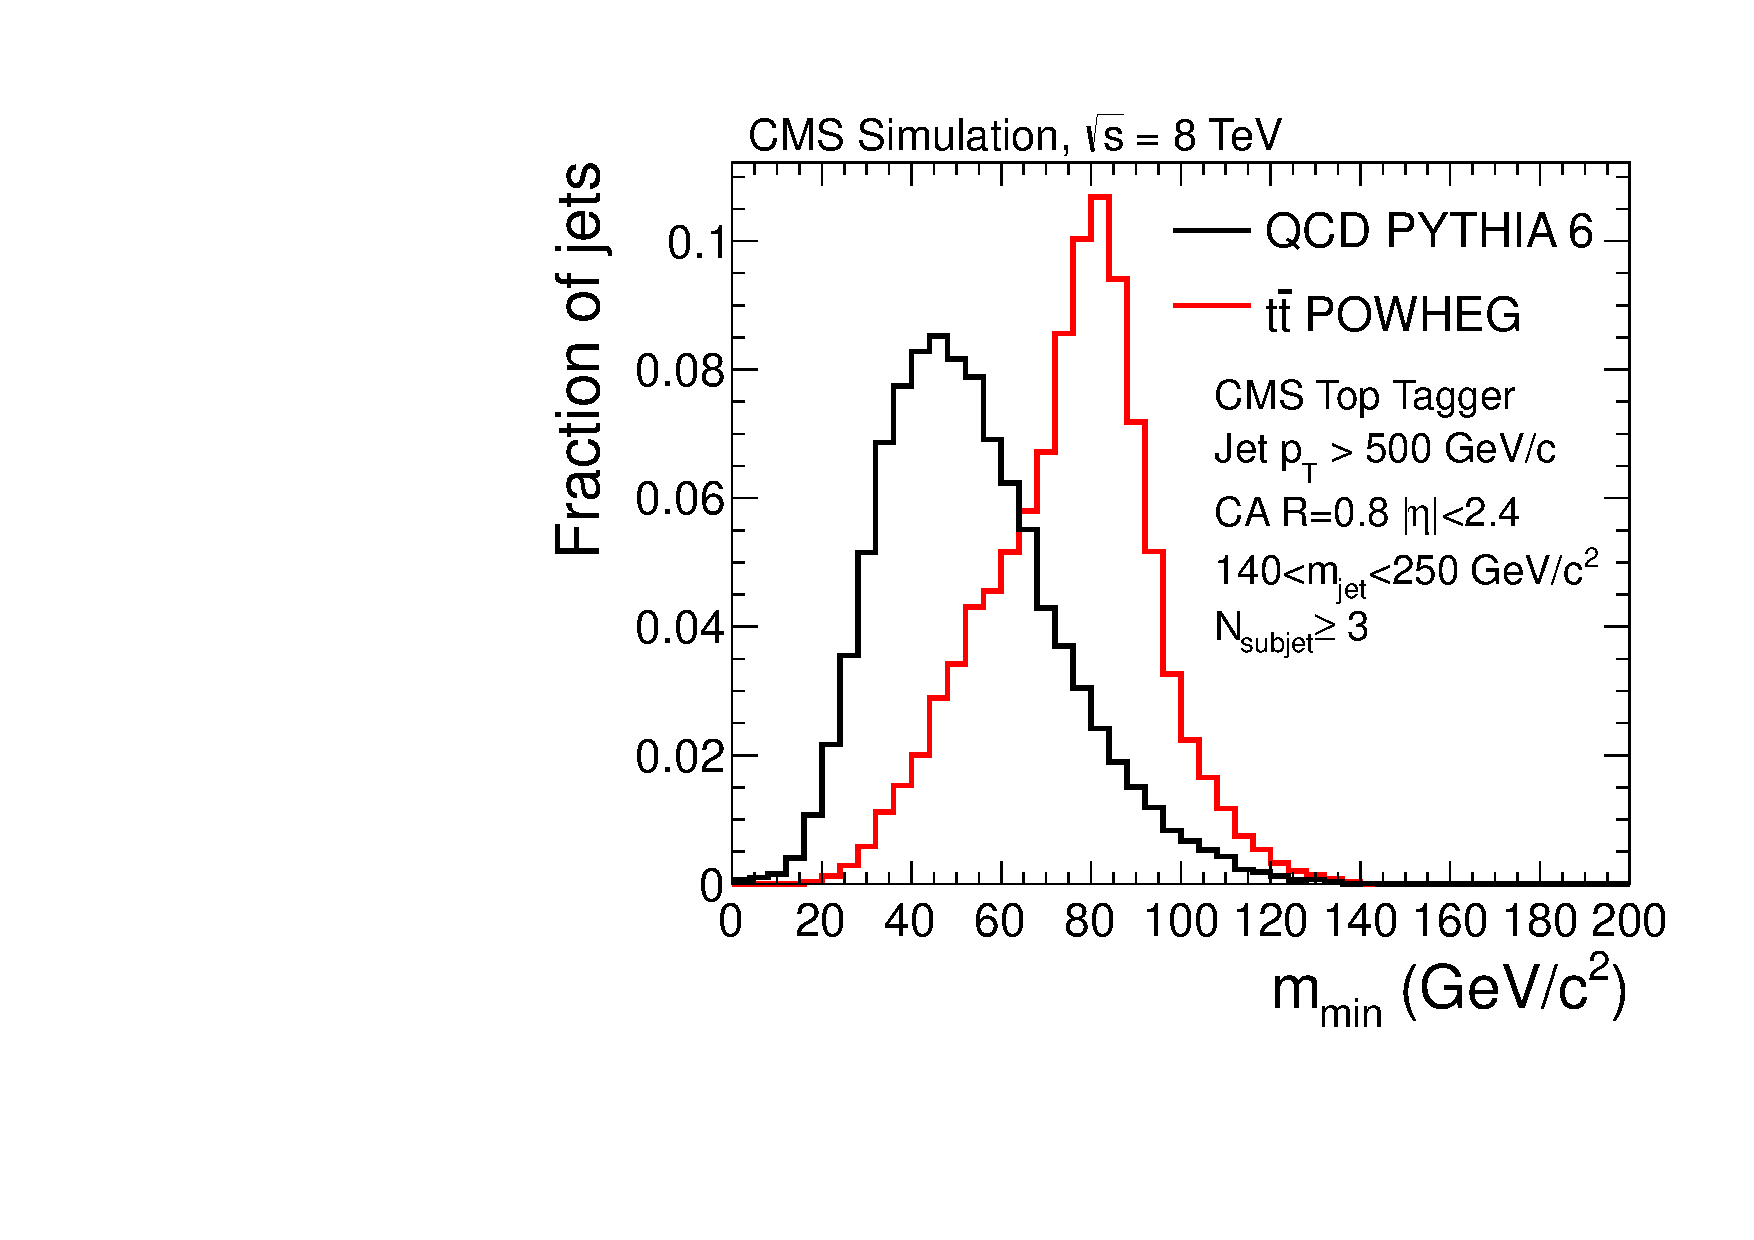
\includegraphics[width=0.49\textwidth]{figures/Draw2HistogramsFrom1File_QQ_MINM_CUT_PT_MASS_NSUB_TT_MINM_CUT_PT_MASS_NSUB_JetPt500.pdf}
  \end{tabular}
  \caption{Jet mass (\textit{left}) and minimum pairwise subjet mass (\textit{right}) for CA8 jets with $\pt > 500$\gev from a simulated $t\bar{t}$ POWHEG sample (red) and from a simulated QCD PYTHIA sample (black). Taken from~\cite{CMS:2014fya}.}
  \label{fig:boosted_top_cms_variables}
\end{figure}
 \item \textbf{CMS Top Tagger:} The CMS Top Tagger~\cite{CMS-PAS-JME-09-001} is based on the Top Tagger developed by Kaplan et al.~\cite{Kaplan:2008ie} and acts on jets clustered by the Cambrigde-Aachen algorithm with distance parameter $\mathrm{R} = 0.8$ (CA8 jet). These jets used as input for the algorithm are denoted as \textit{hard jets}. Since the decay products of the hadronic top are not expected to be all collimated in one jet with $\mathrm{R} = 0.8$ for low transverse momenta, only jets with $\pt^{jet} > 350$\gev are considered. In order to identify subjets within the hard jets, a two stage decomposition procedure is applied. First, the algorithm aims at splitting the hard jet into two subclusters (\textit{primary decomposition}) and second, it is attempted to further split the clusters emerging from the first step (\textit{secondary decomposition}). Hence, the pairwise clustering sequence used to form the hard jet is performed in reverse order to identify subclusters. Typically, subjets are found when they are spatially well separated and carry a significant fraction of the momentum of the hard jet. Details on the actual splitting criteria can be found in~\cite{CMS:2014fya}. With this approach up to four individual subjets are identified within the hard jet. After a successful decomposition procedure kinematic criteria can be applied to the identified subjets in order to tag top jets. In the CMS top-tagging algorithm -- as employed in this thesis -- the following selections are used:
\begin{description}
 \item -- Number of subjets $\ge$ 3
 \item -- The jet mass $m_{\mathrm{jet}}$, i.e. the mass of the four-vector sum of the constituents of the hard jet, has to be close to the top-mass: $m_{\mathrm{jet}} = 140-250$\gev.
 \item -- The invariant mass of each pair of the three subjets highest in \pt is calculated. The minimum of the pairwise masses $m_{\mathrm{min}}$ has to be close to the W mass: $m_{\mathrm{min}} > 50$\gev.
\end{description}
In Fig.~\ref{fig:boosted_top_cms_variables}, the distributions for jet mass and minimum pairwise mass are illustrated for a simulated $t\bar{t}$ (red) and QCD multijet (black) sample at $\sqrt{s} = 8$\tev. 
 \item \textbf{HEP Top Tagger:} The HEP Top Tagger~\cite{Plehn:2010st} uses jets with an even larger distance parameter than the CMS Top Tagger of $R = 1.5$ (CA15 jets). This makes the HEP top-tagging algorithm especially suitable for tops with moderate boost. Fat jets with a transverse momentum greater than 200\gev are used as input for the algorithm. Since a larger jet size is in principle more prone to disturbing effects from the underlying event or pile-up, a sophisticated decomposition procedure is applied to distinuigh hard subjets from soft components. Similar to the decomposition done for the CMS tagger, the identification of subjets is based on going through the cluster history of a jet in reversed order. First, the jet is decomposed into subclusters applying a \textit{mass drop condition} discarding too soft components. Afterwards, all combinations of three clusters resulting from the mass drop decomposition are reclustered into subjets. For each combination the subjets are filterd by keeping only the five subjets highest in \pt. Finally, the combination with the mass determined from the filtered subjets closest to the top mass is kept and reclustered to force three subjets. Details on the mass drop decomposition and reclustering criteria can be found in~\cite{CMS:2014fya}. Kinematic selections are applied to these three final subjets in order to identify the top jets. The following quantities are used based on the invariant mass of combinations of subjets:
\begin{figure}[!tp]
  \centering 
  \begin{tabular}{cc}
    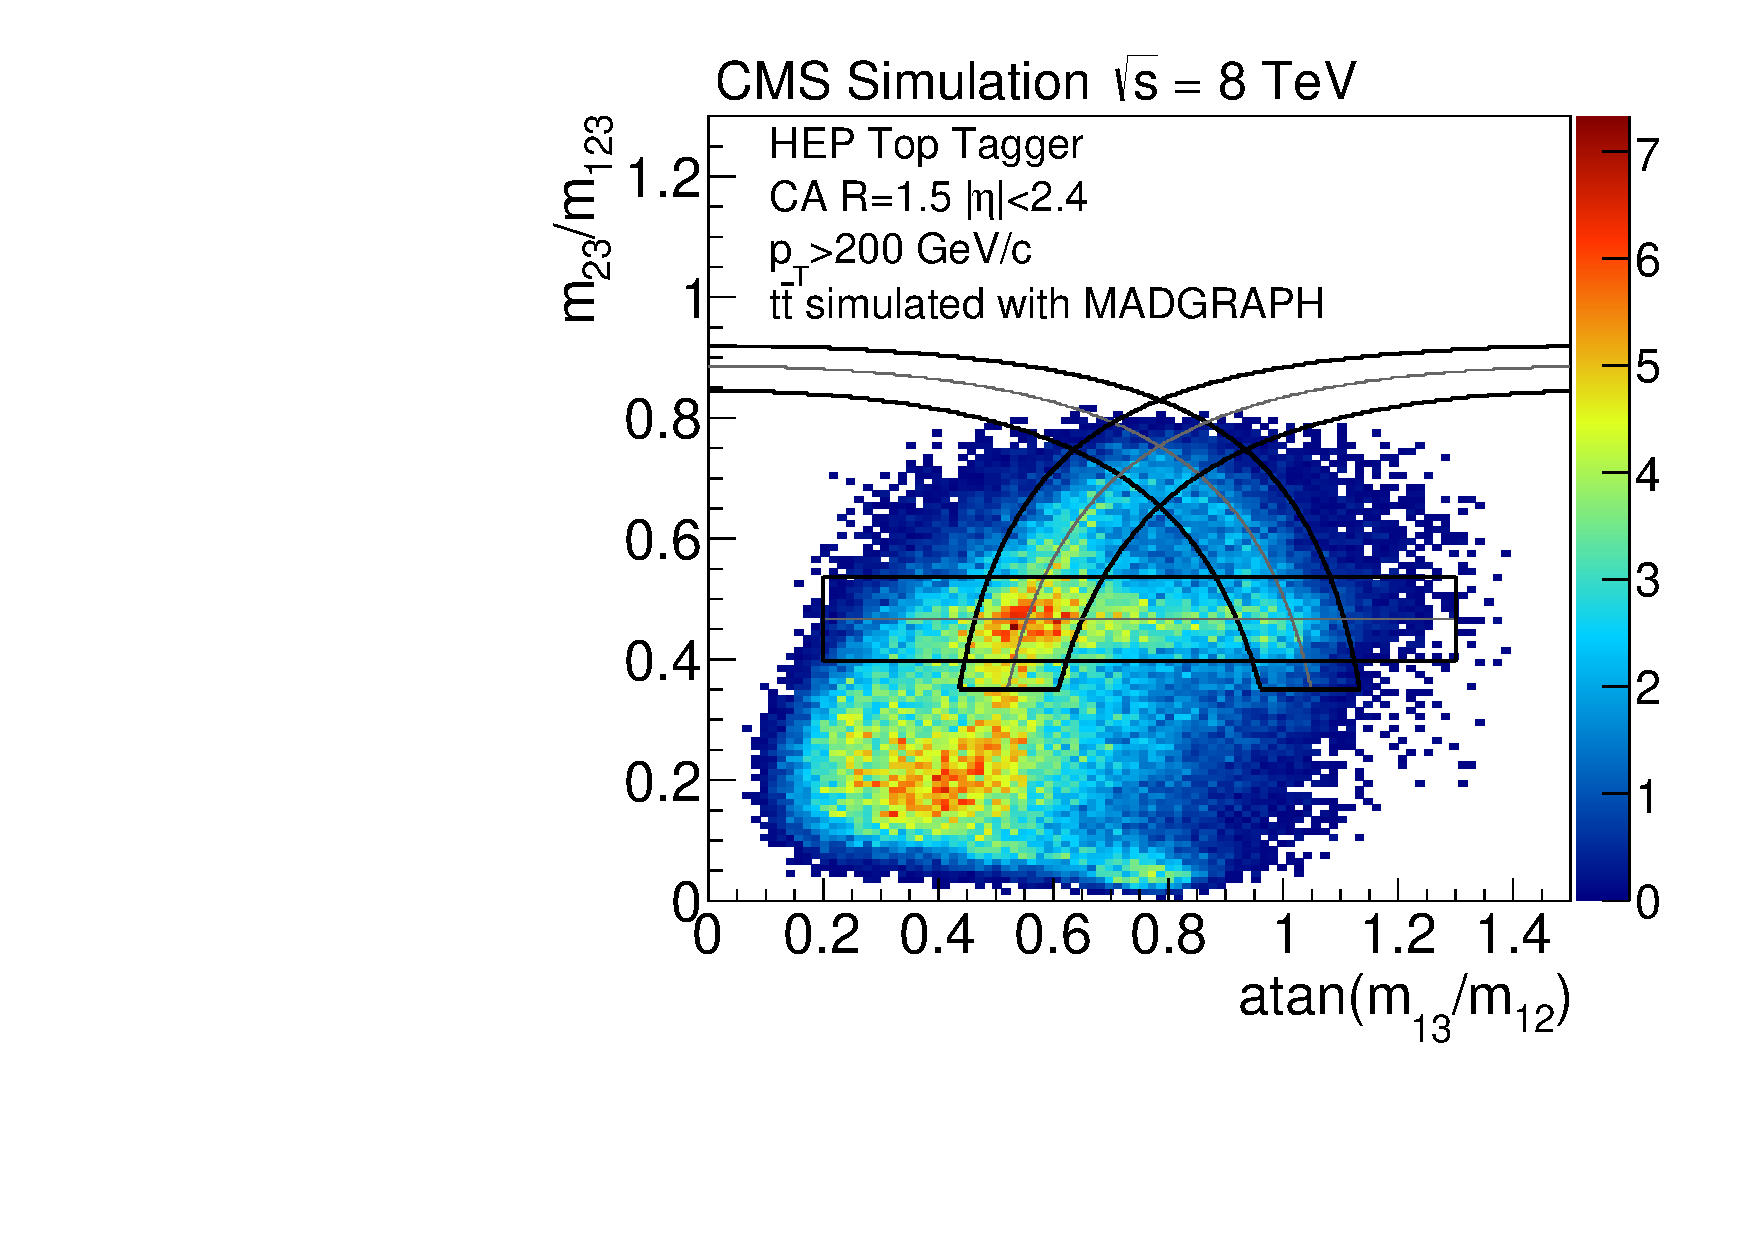
\includegraphics[width=0.49\textwidth]{figures/Pheno2DPlot_HTT2D_NOheptoptag_NOmasscut_hists_Signal_Add.pdf} & 
    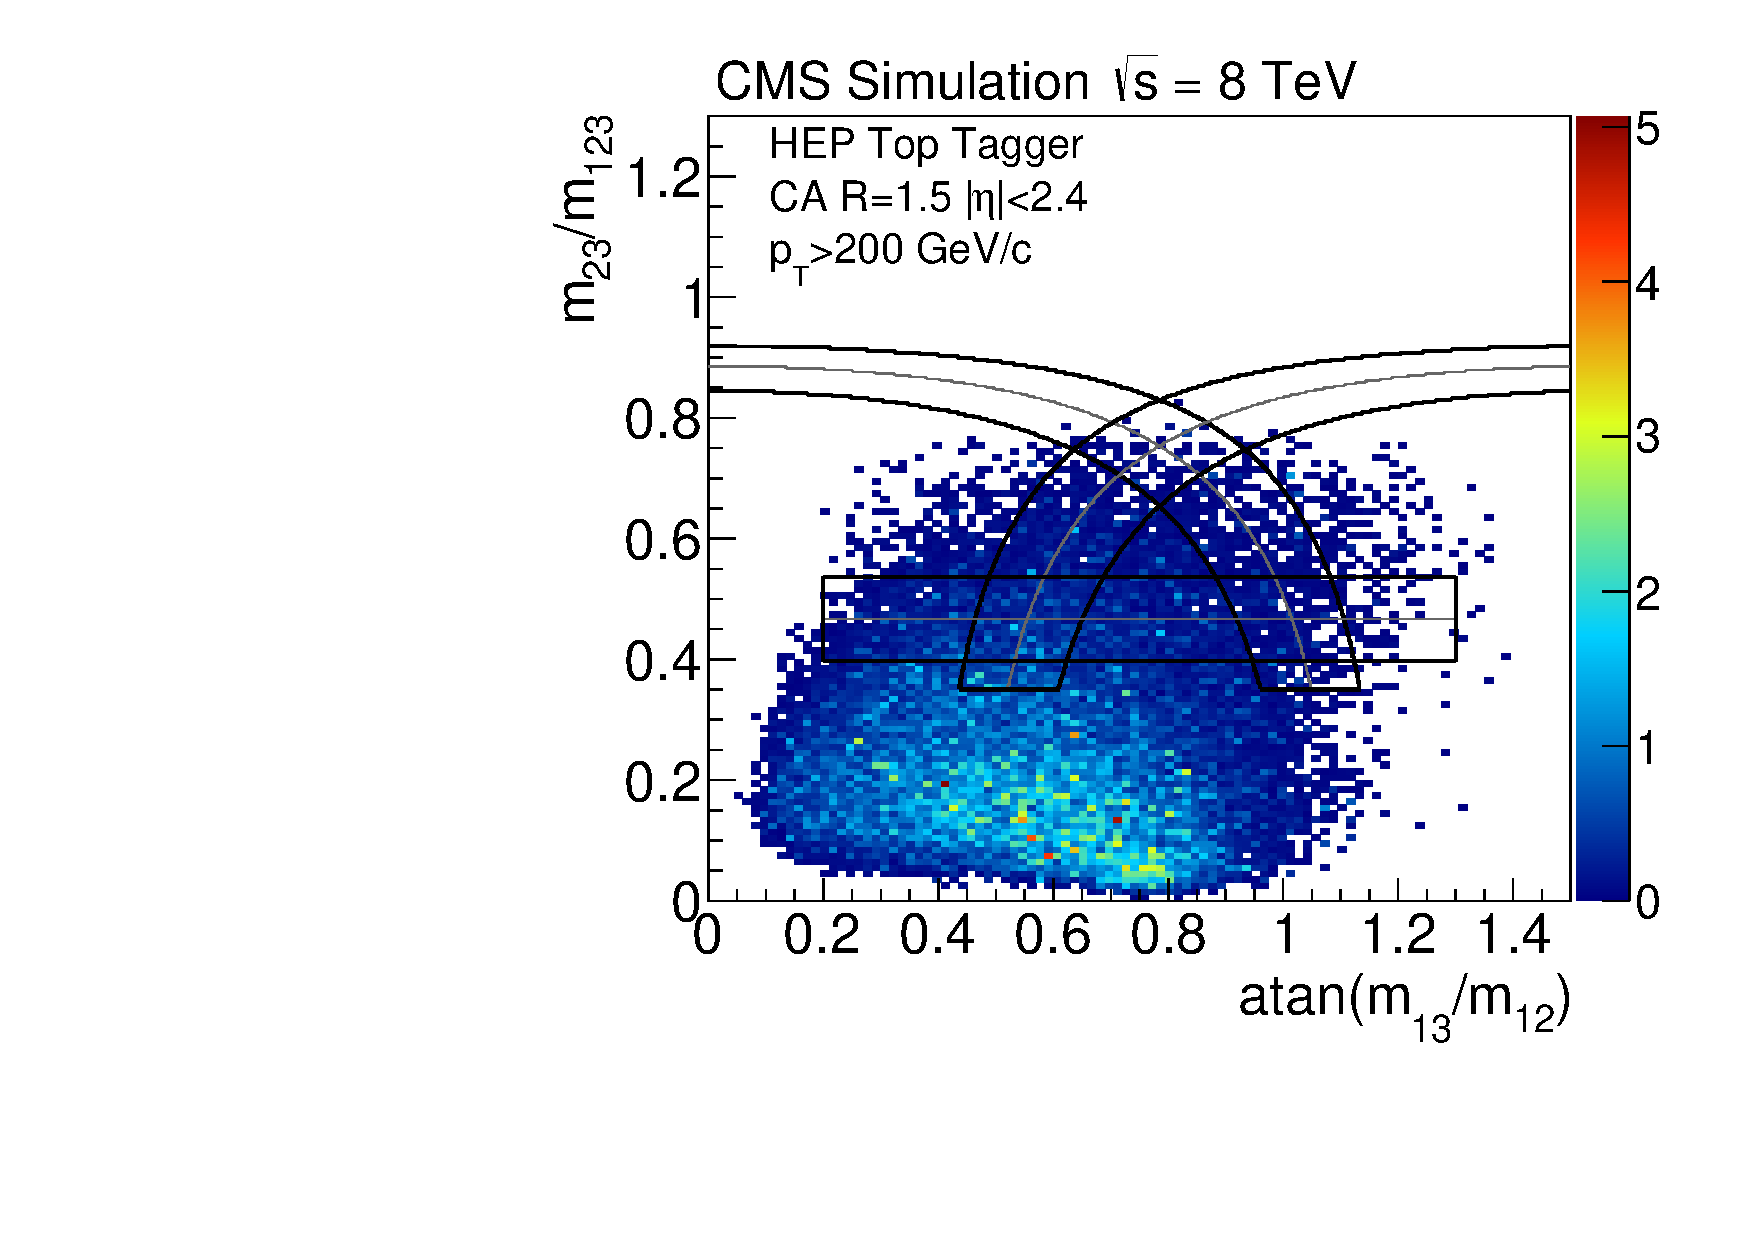
\includegraphics[width=0.49\textwidth]{figures/Pheno2DPlot_HTT2D_NOheptoptag_NOmasscut_hists_Background_Add.pdf}
  \end{tabular}
  \caption{Two-dimensional distributons of $m_{\mathrm{23}}/m_{\mathrm{123}}$ versus $\mathrm{atan}(m_{\mathrm{13}}/m_{\mathrm{12}})$ for HEP Top Tagger subjets from CA15 jets with $\pt > 200$\gev for a simulated $t\bar{t}$ MADGRAPH sample (\textit{left}) and for a simulated background sample composed of cross-section weighted boson + jets, diboson, single-top, $t\bar{t}$ all-hadronic and $t\bar{t}$ leptonic events (\textit{right}). The A-shaped region indicates the selected region by the HEP Top Tagger. Taken from~\cite{CMS:2014fya}.}
  \label{fig:boosted_top_hep_variables}
\end{figure}
\begin{description}
 \item -- The invariant mass of the sum of the four-vectors of the three subjets is required to be in the top mass window: $m_{\mathrm{123}} = 140 - 250$\gev.
 \item -- In order to select the W mass the jet has to satisfy at least one of the following conditions based on the subjet pairwise masses
\begin{description}
 \item \begin{equation*}
0.2 < \mathrm{atan} \frac{m_{\mathrm{13}}}{m_{\mathrm{12}}} < 1.3 \; \; \mathrm{and} \; \; R_{\mathrm{min}} < \frac{m_{\mathrm{23}}}{m_{\mathrm{123}}} < R_{\mathrm{max}}
\end{equation*}
 \item \begin{equation*}
R^2_{\mathrm{min}}(1+(\frac{m_{\mathrm{13}}}{m_{\mathrm{12}}})^2) < 1 - (\frac{m_{\mathrm{23}}}{m_{\mathrm{123}}})^2) < R^2_{\mathrm{max}}(1+(\frac{m_{\mathrm{13}}}{m_{\mathrm{12}}})^2) \; \; \mathrm{and} \; \; \frac{m_{\mathrm{23}}}{m_{\mathrm{123}}} > 0.35
\end{equation*}
 \item \begin{equation*}
R^2_{\mathrm{min}}(1+(\frac{m_{\mathrm{12}}}{m_{\mathrm{13}}})^2) < 1 - (\frac{m_{\mathrm{23}}}{m_{\mathrm{123}}})^2) < R^2_{\mathrm{max}}(1+(\frac{m_{\mathrm{12}}}{m_{\mathrm{13}}})^2) \; \; \mathrm{and} \; \; \frac{m_{\mathrm{23}}}{m_{\mathrm{123}}} > 0.35
\end{equation*}
\end{description}
where the indices of $m$ indicate the rank of the considered subjets with respect to the transverse momentum, $R_{\mathrm{min}} = (1 - f_{W}) \times m_W/m_t$ and $R_{\mathrm{max}} = (1 + f_{W}) \times m_W/m_t$ for the W mass width chosen to be $f_W = 0.495$.  
\end{description}
The criteria related to the selection of the W mass are illustrated in Fig.~\ref{fig:boosted_top_hep_variables} for signal events as well as background events and indicated by the black solid lines resulting in an A-shaped region.
\end{description}
In analogy to the b-tagging algorithms, different working points for each top tagger can be defined characterized by a specific top-tag efficiency and misidentification rate. Typically, the working points are chosen such that they have a minimum mistag rate for a given signal efficiency. Commonly, the top-tag efficiency for simulated events is defined as the number of jets passing the top-tagging selection divided by the number of jets spatially matched to a simulated hadronic top or anti-top passing a certain \pt selection. Similarly, the mistag rate is defined as the number of jets passing the top-tagging selection divided by the number of jets spatially matched to a simulated quark or gluon from the hard process passing the \pt selection. The top-tag efficiency determined from simulated $t\bar{t}$ POWHEG events for the selection criteria described above amounts to 35.3\% for a matched parton-\pt of $> 200$\gev for the HEP Top Tagger and 38.3\% for a matched parton-\pt of $> 400$\gev for the CMS Top Tagger while the mistag rates as determined from simulated PYTHIA QCD multijet events are 2.6\% and 2.5\%, respectively. However, these efficiencies and mistag rates show a moderate dependence on pile-up such that in high pile-up environments a performance degradation is expected. For instance, in the case of the CMS Top Tagger the efficiency decreases as function of the number of primary vertices with a slope of $0.031\% \pm 0.034\%$ while the mistag rate increases with a slope of $0.095\% \pm 0.006\%$.      

%\subsection{Subjet B-Tagging}
%\label{sec:boosted_tops_subjet_b}

%\subsection{N-subjettiness}
%\label{sec:boosted_tops_n_subjettiness}
